\section{Konstruktion}
\label{sec:konstruktion}

\begin{figure}
    \centering
    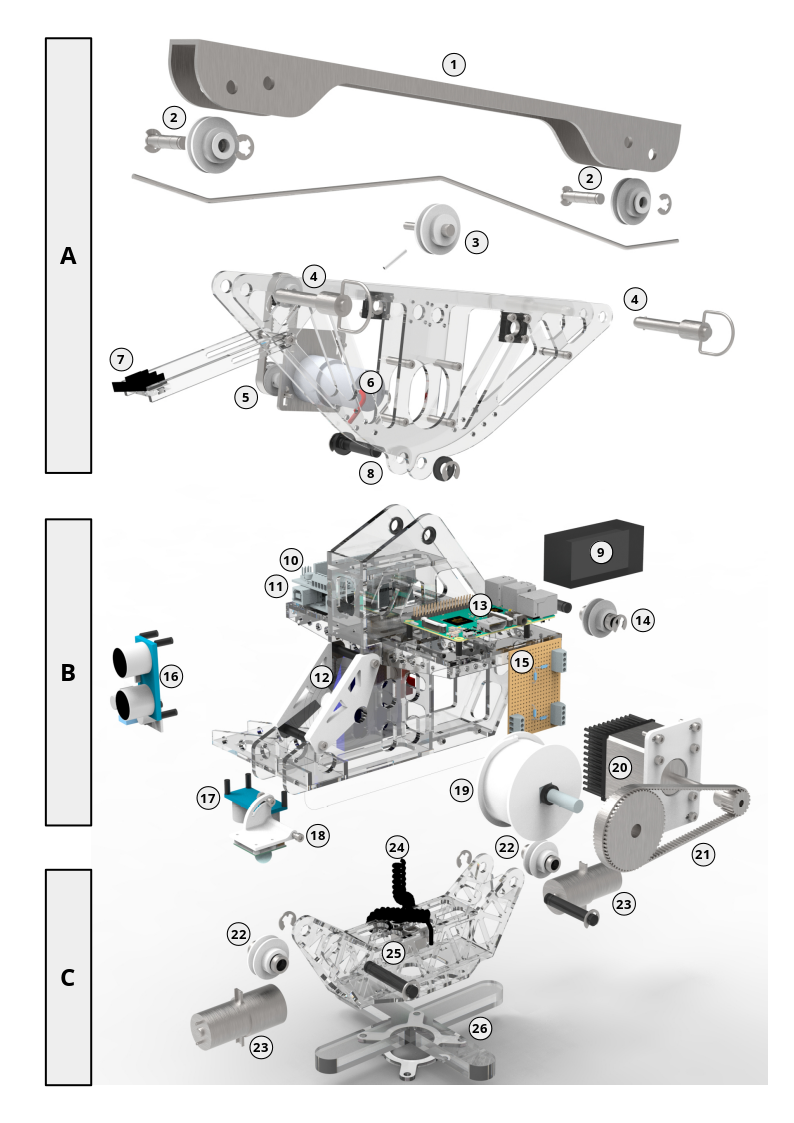
\includegraphics[width=1.0\linewidth]{graphs/beschriftung.png}
    \caption{Die Explosionsansicht des CAD-Modells von \textit{Silisloth} mit nummerierten Komponenten}
    \label{fig:explosionsansicht}
\end{figure}

Die Konstruktion von \textit{Silisloth} (\imgref{fig:explosionsansicht}) folgt weitgehend den CAD-Plänen von PREN 1 \cite[S. 12-13]{pren1}. Einige Teile sind dazugekommen (Endschalter, PCB), manche Teile wurden anders positioniert (Ultraschallsensor in x-Richtung, Luftpumpen und Magnetventil) und in manchen Bereichen wurde die Konstruktion verfeinert und optimiert (Greifeinheit, Kontrollbox). Die Konstruktion lässt sich in drei Bereiche unterteilen und besteht aus den folgenden Komponenten:

\begin{multicols}{2}

\textsc{A: Aufhängung}

\begin{enumerate}
    \item Halterungsschiene für Aufhängung
    \item Laufrollen mit Bolzen
    \item Antriebsrad
    \item Quick-Pins zur Befestigung
    \item Riemengetriebe für den Antrieb (Übersetzung)
    \item Getriebemotor für den Antrieb
    \item Endschalter
    \item Bolzen zur Befestigung der Kontrollbox
\end{enumerate}

\textsc{B: Kontrollbox}

\begin{enumerate}
\setcounter{enumi}{8}
    \item LiPo-Akku (Laststromkreis)
    \item Motor Shield
    \item Arduino
    \item LiPo-Akku (Steuerstromkreis) mit USV (verborgen)
    \item Raspberry Pi
    \item Laufrolle für Hubmechanismus
    \item PCB für Ultraschallsensoren
    \item Ultraschallsensor in x-Richtung
    \item Ultraschallsensor in z-Richtung
    \item Raspi-Cam (neigbar)
    \item Seiltrommel
    \item Schrittmotor mit Kühlkörper
    \item Riemengetriebe für den Hubmechanismus (Untersetzung)
    \item Laufrollen für Seilwinde
\end{enumerate}

\textsc{C: Greifmechanismus}

\begin{enumerate}
\setcounter{enumi}{22}
    \item Luftpumpen
    \item Spiralkabel
    \item Magnetventil
    \item Silikongreifer
\end{enumerate}

\end{multicols}

In den folgenden Abschnitten wird erläutert, auf welche Eigenschaften bei der Umsetzung besonderen Wert gelegt wurde, und wie dabei die Designentscheide gefällt wurden.

\subsection{Kontrollbox}

Während der konstruktiven Phase wurde besonderen Wert auf die Designeigenschaften Zugänglichkeit und Kompaktheit gelegt. Es sollte gewährleistet sein jederzeit auf alle Komponenten zugreifen zu können, damit an diesen, wenn nötig, Eingriffe vorgenommen werden können, ohne dass eine Demontage nötig oder Betriebsunterbrüche daraus resultieren würden. Es wurde speziell darauf geachtet Stapelung von Komponenten zu vermeiden.

In Bezug auf die Kompaktheit wurde besonders auf platzsparendes Design, einfache Transportierbarkeit und ein geringes Gewicht geachtet.

Beim Seilwindenmotor war während der Designphase nicht sicher, ob dieser den Anforderungen genügt. Deshalb wurde hier eine Adapterplatte eingesetzt, sodass nur diese Platte und nicht eine ganze Komponente ausgetauscht werden müsste, sollte ein anderer Seilwindenmotor zum Einsatz kommen. Zusätzlich wurde die Adapterplatte mit Langlöchern versehen, womit sich der Achsenabstand leicht variieren lässt. Dies dient einerseits dem Toleranzausgleich und andererseits zum Spannen des Riemens.

Grosser Wert wurde bei der Konstruktion darauf gelegt, dass der Schwerpunkt an der richtigen Stelle zu liegen kommt, sodass der Verbindungsbolzen und der Schwerpunkt der Kontrollbox zusammen mit dem Greifmechanismus im Lot sind. Dies setzte voraus, dass das Einzelgewicht aller Komponenten bekannt bzw. die Dichte aller Materialien hinterlegt war. Deshalb mussten zunächst alle Kaufteile beschafft werden, bevor die Kontrollbox gelasert werden konnte.

Für die finale Justierung wurde die Konstruktion so gewählt, dass der Akku in x-Richtung leicht variabel verbaubar ist, was einen gewissen Korrekturspielraum zulässt.

Dieser Ansatz wurde gewählt, damit für die Sensorikelemente (Ultraschallsensoren) mit einer geringen Toleranzbreite gearbeitet werden konnte. So konnte zusätzlich die Anzahl möglicher Fehl- oder Störquellen bei den Sensoren minimiert werden. Bei der Kamera war der optimale Blickwinkel noch nicht bekannt. Deshalb fiel die Wahl bewusst auf eine einstellbare Halterung, die sich um $75\degree$ an der y-Achse rotieren lässt.

\subsection{Greifmechanismus}

Der Greifmechanismus ist symmetrisch um die x-z-Ebene und die y-z-Ebene aufgebaut. Damit liegt der Schwerpunkt in seinem Zentrum, wodurch gewährtleistet ist, dass der Mechanismus jederzeit horizontal, und der Silikongreifer optimal ausgerichtet ist.

Bei der Konstruktion des Greifmechanismus wurde auf einen kompakten Aufbau geachtet, damit die Perspektive der Kamera möglichst wenig eingeschränkt wird. Auch diese Konstruktion folgt der Leichtbauweise, sodass der Seilwindenmotor mit dem Hubmechanismus nicht am Limit betrieben werden muss.

Um die Stabilität des Greifers zu gewährleisten, wurde eine Halterung konstruiert. Zwei Platten halten den Greifer zusammen. Greifer, Platten, Luftpumpen, Magnetventil, Umlenkrollen und unteres Gerüst bilden den Greifmechanismus.

Der Silikongreifer wird mit zwei $12V$-Luftpumpen aufgeblasen. Bei den ersten Versuchen wurde festgestellt, dass eine Pumpe alleine den Greifer nicht genug schnell mit Luft füllt. Bei zwei Pumpen wurde dann die gewünschte Griff-Geschwindigkeit erreicht.

Damit der Luftstrom gesteuert werden kann, ist ein Magnetventil zwischen Luftpumpen und Silikongreifer geschaltet. Somit kann die Luft zu einem gewünschten Zeitpunkt aus dem Greifer weggeführt werden.

Um die Dichtheit zu testen, wurde der Greifer mit Luft gefüllt und ein Würfel eingeklemmt. Der Greifer hielt den Würfel über vier Minuten in der Luft, somit erfüllte er die Anforderungen. Die Herstellung des Silikongreifers wurde bereits in der Dokumentation von PREN 1 \cite[S. 44-46]{pren1} beschrieben.

\subsection{Weitere Aspekte der Konstruktion}

\begin{description}
    \item[Fortbewegung] Das treibende, sich in der Mitte der Aufhängung befindende Kunststoffrad wird über einen Zahnriemen von einem Getriebemotor angetrieben. Das Antriebsrad befindet sich unterhalb des Stahlseils, damit mehr Normalkraft für die Kraftübertragung (Reibung) gewonnen werden kann. Zwei zusätzliche, nicht angetriebene Kunststoffräder, welche sich oberhalb des Seils befinden, stützen die Laufkatze. Die Räder sind auf Stahlwellen befestigt, welche wiederum in Kugellagern laufen, um einen möglichst geringen Reibungsverlust zu erzielen.
    \item[Berechnung für die Wellenabstände] Die Berechnung für die Wellenabstände, welche für die Aufhängung und Kontrollbox verwendet wird, erfolgt über die \calcrefplain{eq:wellenabstand} \cite[Kapitel 16, Formel 22]{roloff-matek}.
    \item[Polyvalenz] In der Testphase hat sich gezeigt, dass das Konzept mit dem Silikongreifer multiple Einsatzmöglichkeiten bietet. Diese polyvalenten Greifer, die einer menschlichen Hand ähnlich sind, können für verschiedenste Objekte mit unterschiedlichen Geometrien und aus verschiedenen Materialien eingesetzt werden. Diese Polyvalenz zeigt sich auch beim Flaschenzug, da sich der Einsatz im Längenbereich fast beliebig erweitern lässt.
    \item[Gewicht] Mit der Leichtbauweise wurde das Ziel der Kompaktheit erreicht -- unter anderem mit Erleichterungslöchern und Fachwerkstrukturen.
    \item[Mehrfachverwendung] Der Herstellungs- und Designaufwand wurde durch gezielte Mehrfachverwendung von Komponenten reduziert. Zum Beispiel wurde für die drei Seilumlenkrollen des Hubmechanismus dreimal das gleiche Konzept mit den gleichen Bauteilen verwendet, d.h. identische Rollen, Lagerungs- und Sicherungselemente.
    \item[Symmetrie] Bei der Konstruktion der tragenden Strukturelemente wurde auf Symmetrie geachtet, sodass Teile gespiegelt oder mehrfach verwendet werden konnten. Dadurch liess sich der Konstruktionsaufwand optimieren. Symmetrie hat auch einen positiven Effekt auf den Schwerpunkt.
    \item[Verwendete Materialien] Die verwendeten Materialien sind Acrylglas der Stärken drei und vier Millimeter. Die etwas komplexeren Teile wurden aus Acrylnitril-Butadien-Styrol (ABS) 3D gedruckt. Für die Wellen und Achsen fiel die Wahl auf S235-Stahl.
    \item[Montage] Im CAD-Prozess wurde bewusst ein sehr hoher Detaillierungsgrad der einzelnen Teile angestrebt, sodass bei der Montage der Kaufteile keine Nachbearbeitung nötig war. Dies geschah auch zum Schutz der Komponenten, die durch solche Eingriffe beeinträchtigt worden wären.
\end{description}

\begin{align}
    e   &\approx \frac{L_d}{4} - \frac{\pi}{8} \cdot (d_{dg} + d_{dk}) + \sqrt{\left[\frac{L_d}{4}-\frac{\pi}{8} \cdot (d_{dg} + d_{dk})\right]^2 - \frac{(d_{dg}-d_{dk})^2}{8}} \label{eq:wellenabstand} \\
    e   &= \text{Wellenabstand} \nonumber \\
    L_d &= \text{Zahnriemenlänge (Zähnezahl Riemen multipliziert mit dessen Teilung)} \nonumber \\
    d_{dg}, d_{dk} &= \text{Scheibendurchmesser kleines bzw. grosses Rad} \nonumber
\end{align}

\begin{figure}[H]
    \centering
    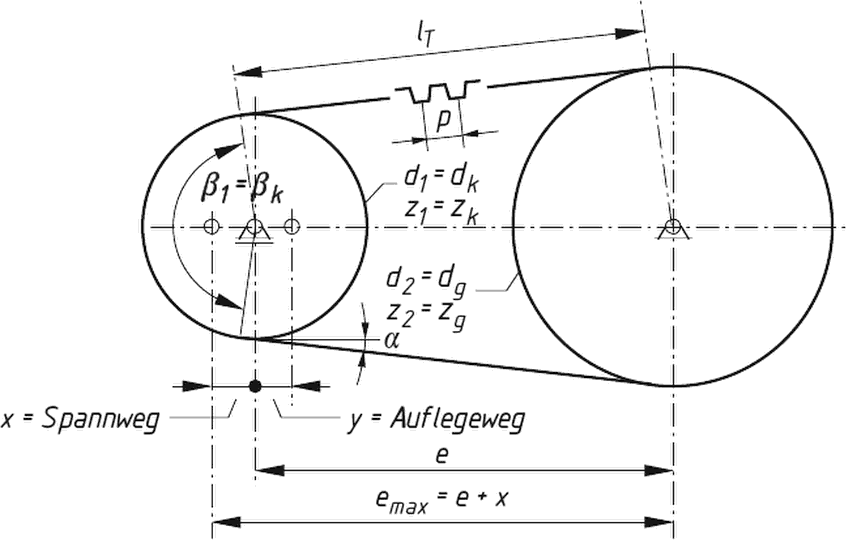
\includegraphics[width=0.7\linewidth]{pics/riemengetriebe.png}
    \caption{Die Berechnung des Wellenabstands $e$ \protect\cite[S. 206]{roloff-matek}}
    \label{fig:riemengetriebe}
\end{figure}
